% A shear does not change the area of a parallelogram (Cavalieri).
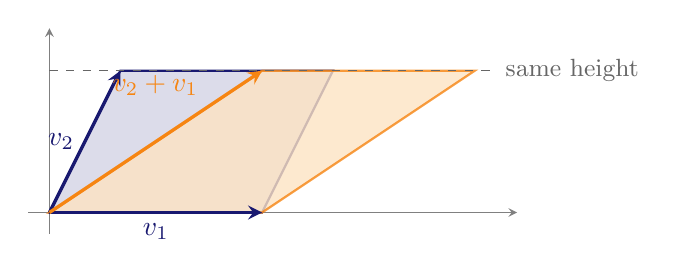
\begin{tikzpicture}[scale=0.9,>=stealth]
\draw[->,black!50] (-0.3,0) -- (6.6,0); \draw[->,black!50] (0,-0.3) -- (0,2.6);
\filldraw[fill=MidnightBlue!15,draw=MidnightBlue,thick] (0,0) -- (3,0) -- (4,2) -- (1,2) -- cycle;
\filldraw[fill=BurntOrange!20,draw=BurntOrange,thick,opacity=0.8] (0,0) -- (3,0) -- (6,2) -- (3,2) -- cycle;
\draw[->,very thick,MidnightBlue] (0,0) -- (3,0) node[midway,below] {$v_1$};
\draw[->,very thick,MidnightBlue] (0,0) -- (1,2) node[midway,left] {$v_2$};
\draw[->,very thick,BurntOrange] (0,0) -- (3,2) node[pos=0.75,above left] {$v_2+v_1$};
\draw[dashed,black!60] (0,2) -- (6.3,2); \node[right,black!60,font=\small] at (6.3,2) {same height};
\end{tikzpicture}
